\section{Empirical Strategy}

 \frame{\sectionpage}

    \begin{frame}{Randomization Test}
        \only<1>{
            $$168\text{\ audited after election }v.s.\ 205\text{ audited before election}$$
        }

        \only<2>{
            $$\underbrace{168}_{\color{orange}C}\text{\ audited after election }v.s.\ \underbrace{205}_{\color{orange}T}\text{ audited before election}$$
        }
    \end{frame}
    
    \begin{frame}{Randomization Test: Political Characteristics}
        \only<1->{
            $$\underbrace{168}_{\color{orange}C}\text{\ audited after election }v.s.\ \underbrace{205}_{\color{orange}T}\text{ audited before election}$$
        }

        \uncover<1->{
        \begin{table}[h!]
            \footnotesize
            \begin{center}
              \label{tab:randomization1}
              \begin{tabular}{lcccc}
                
                & Control & Treatment & Difference & Std.Error \\
                \hline
                \textcolor<2>{orange}{Reelection rates: 2004 elections} & 0.413 & 0.395 & 0.018 & 0.045 \\
                \textcolor<3-4>{orange}{Reelection rates: 2000 elections \only<4>{(669 manicipalities)}} & 0.423 & 0.443 & -0.020 & 0.040 \\
                \textcolor<5>{orange}{2004 reelection rates, conditional on running} & 0.585 & 0.559 & 0.026 & 0.044 \\
                \textcolor<5>{orange}{Ran for reelection in 2004} & 0.707 & 0.707 & -0.001 & 0.060\\
                \textcolor<6>{orange}{Mayor's vote share in 2000} & 0.529 & 0.525 & 0.004 & 0.013
              \end{tabular}
            \end{center}
          \end{table}
        }
        
    \only<3-4>{
        No significant differences between C and T w.r.t. \textcolor<4>{orange}{\textit{natural}} reelection rates (among those eligible to re-run)
    }

    \only<4>{
        \footnotesize In 2000, every mayor was eligible to run for a second term, since only after 1997 it was allowed to run as an incumbent.
    }

    \only<5>{
        Balanced rate of re-running and incumbent advantage
    }

    \only<6>{
        Initial popularity of reelection seeking mayors is balanced too
    }

    \end{frame}

    \begin{frame}{Randomization Test: Mayor and Municipal Characteristics}
        \only<1->{
            $$\underbrace{168}_{\color{orange}C}\text{\ audited after election }v.s.\ \underbrace{205}_{\color{orange}T}\text{ audited before election}$$
        }

        \uncover<1->{
        \begin{table}[h!]
            \footnotesize
            \begin{center}
              \label{tab:randomization2}
              \begin{tabular}{lcccc}
                
                & Control & Treatment & Difference & Std.Error \\
                \hline
                \multicolumn{5}{l}{\textit{Panel A: Mayor characteristics}}\\
                Member of PMDB & 0.254 & 0.172 & \textcolor<2>{orange}{0.082} & \textcolor<2>{orange}{0.047} \\
                &\\
                \multicolumn{5}{l}{\textit{Panel B: Municipal characteristics}}\\
                Number of newspapers & 3.58 & 2.21 & \textcolor<2>{orange}{1.37} & \textcolor<2>{orange}{0.79} \\
                Share of HHs that own a radio & 0.423 & 0.443 & -0.020 & 0.040 \\
                \textcolor<3>{orange}{Municipalities with a radio station} & 0.585 & 0.559 & 0.026 & 0.044 \\
                \textcolor<3>{orange}{Number of radio stations (condtional on having one)} & 0.707 & 0.707 & -0.001 & 0.060
              \end{tabular}
            \end{center}
          \end{table}
        }

        \only<3>{
        Radio presence is well-balanced.
        }

    \end{frame}

    \begin{frame}{Randomization Test: Constructed Corruption Measure}
        \only<1->{
            $$\underbrace{168}_{\color{orange}C}\text{\ audited after election }v.s.\ \underbrace{205}_{\color{orange}T}\text{ audited before election}$$
        }

        \uncover<1->{
        \begin{table}[h!]
            \footnotesize
            \begin{center}
              \label{tab:randomization3}
              \begin{tabular}{lcccc}
                
                & Control & Treatment & Difference & Std.Error \\
                \hline
                Number of corrupt violations & 1.952 & 1.584 & 0.369 & 0.357 \\
                Total resources audited (R\$) &  5,770,189 & 5,270,001 & 500,188 & 1,361,431
              \end{tabular}
            \end{center}
          \end{table}
        }

        \only<2>{
        The constructed measure is balanced, so is the \textit{intensity} of auditing.
        }

    \end{frame}
    
    
    \begin{frame}{Randomization Test: Constructed Corruption Measure}
        \begin{figure}\label{fig2}
            \centering
            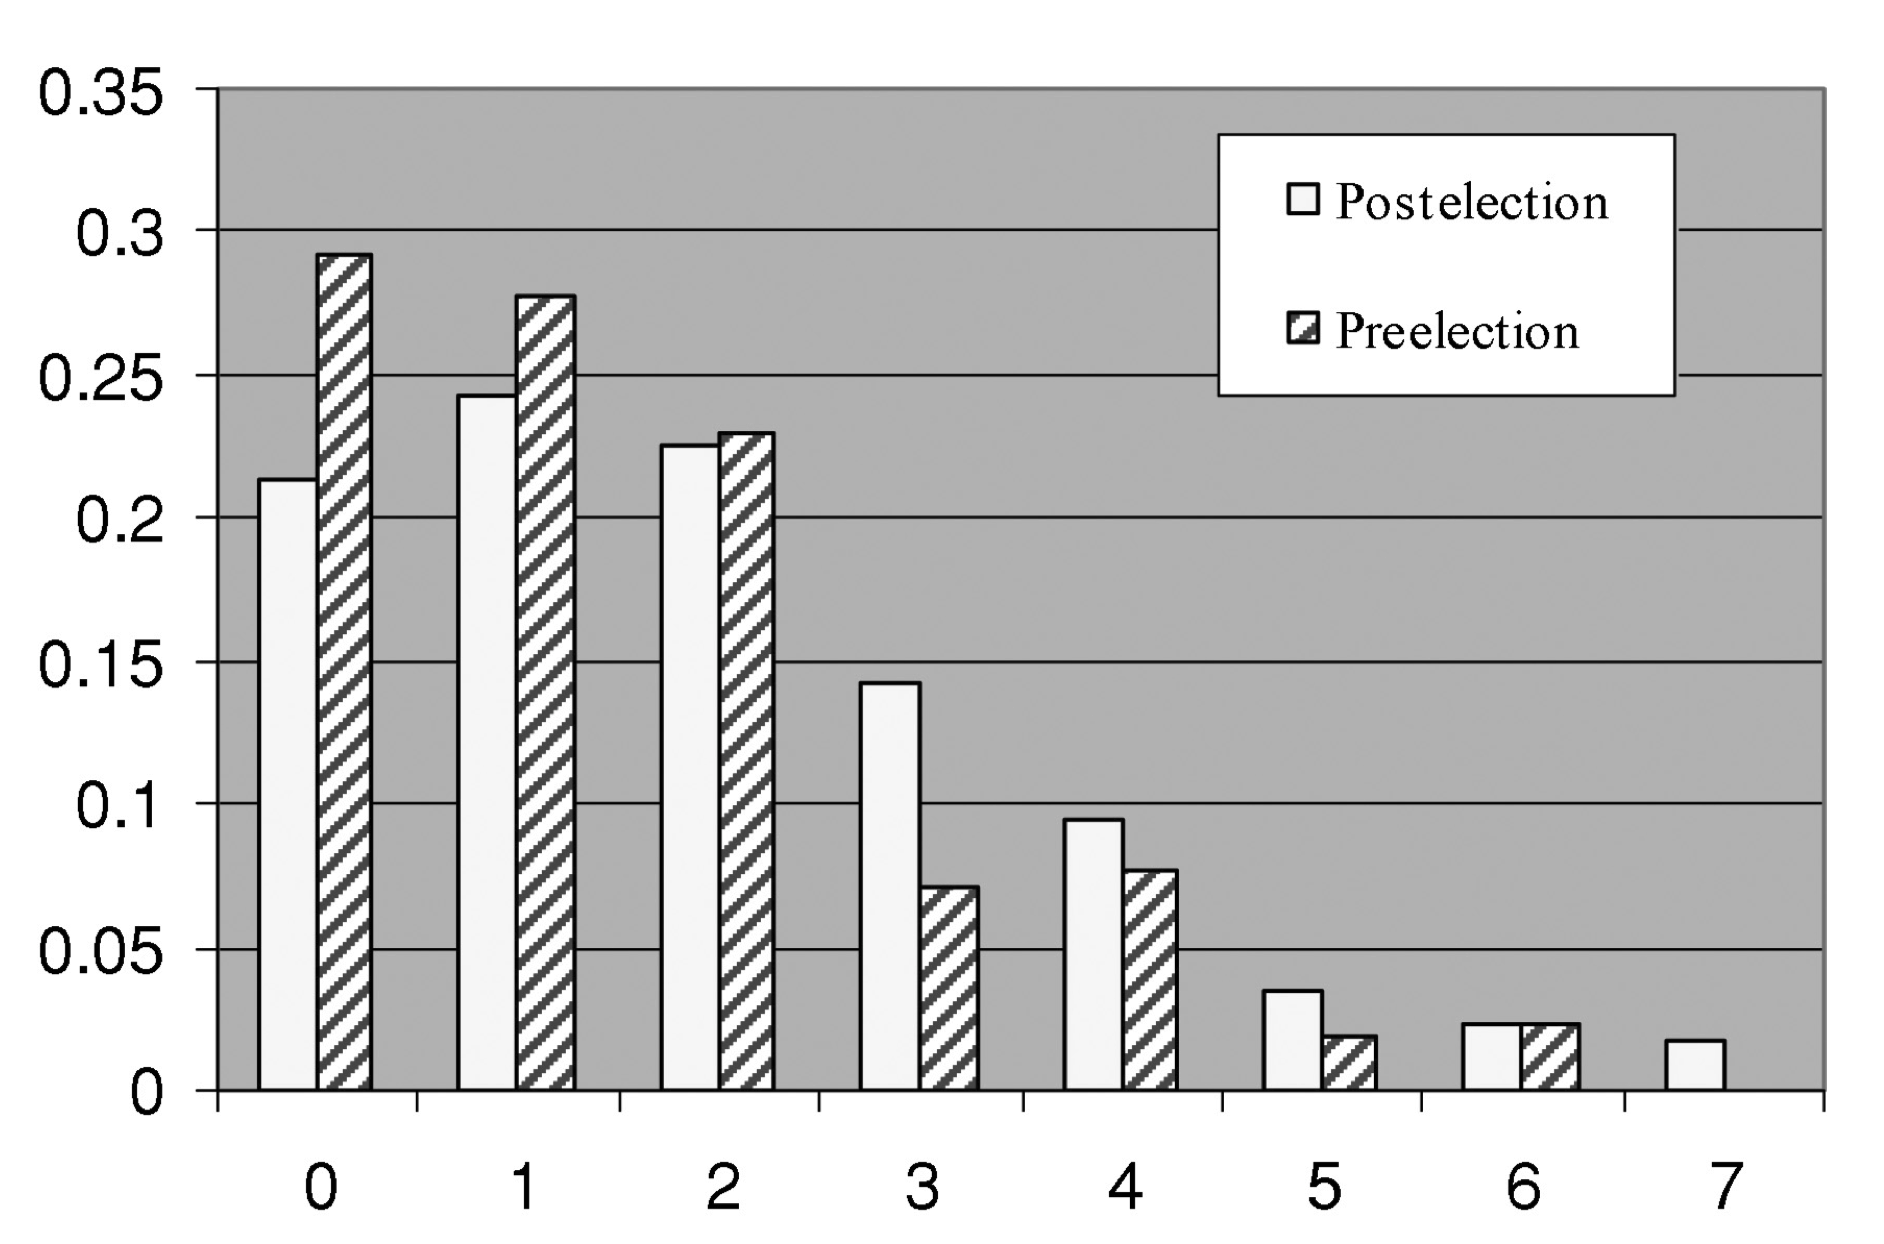
\includegraphics[height = 0.65 \textheight]{images/fig2.png}
            \caption{Distribution of Corrupt Violations}
            \end{figure}
    \end{frame}

\begin{frame}{Estimation I: Exogenous Treatment}
\only<1->{
    \begin{equation*}
        \textcolor<2-3>{orange}{E_{ms}} = \alpha + \textcolor<7>{orange}{\beta} \textcolor<4>{orange}{A_{ms}} + \textcolor<5>{orange}{X_{ms}}\gamma + \textcolor<6>{orange}{\nu_s}+ \epsilon_{ms}
    \end{equation*}
}

\only<2->{
    where:
    \begin{itemize}
        \small
        \item<2-> {\color{orange} $E_{ms}$}: reelection performance of an eligible incumbent mayor in {\color{orange}\textbf{municipality} $m$}, {\color{orange}\textbf{state} $s$}
        \only<3>{
            \begin{itemize}
                \footnotesize
                \item[-] Discrete: whether winning the reelection or not
                \item[-] Continuous: vote share; win margin
                \item[-] Changes from 2000 results: $\Delta E_{ms}=E_{ms,2004}-E_{ms,2000}$
            \end{itemize}
        }
        \item<4-> {\color{orange} $A_{ms}$}: $=1$ if audited prior to the 2004 elections
        \item<5-> {\color{orange} $X_{ms}$}: municipality and mayor controls
        \item<6-> {\color{orange} $\nu_s$}: state fixed effect 
    \end{itemize}
}

\only<7>{
    {\color{orange} $\beta$}: the treatment effect of \underline{being audited and the public release of auditing results}
}
    
\end{frame}

\begin{frame}{Estimation II: Adding Voters' Prior Beliefs}
    \only<1->{
    \begin{equation*}
        E_{ms} = \alpha + \only<2->{ \beta_0 \textcolor<3>{orange}{C_{ms}} +} \beta_1 A_{ms} \only<2->{+ \textcolor<4->{orange}{\beta_2} \textcolor<3>{orange}{\left(A_{ms}\times C_{ms}\right)} } + X_{ms}\gamma + \nu_s + \epsilon_{ms}
    \end{equation*}
    }
    
    \only<3->{
    where:
    \begin{itemize}
        \small
        \item<3-> {\color{orange} $C_{ms}$}: {\color{orange}\textbf{number of}} corrupt irregularities in the municipality
        \item<3-> {\color{orange} $A_{ms}\times C_{ms}$}: interaction term 
    \end{itemize}

}

\only<4->{
    {\color{orange} $\beta_2$}: the treatment effect conditional on corruption levels
    \only<5->{
        \begin{itemize}
            \small
            \item<5-> \textbf{\color{orange}Prediction}: Negative treatment effect at higher levels of reported corruption, presumably positive at lower levels.
            \item<6> \textbf{\color{orange}Underlying assumption}: Voters do \textbf{\color{orange}not} systematically over- or underestimate the incumbent's corruption level.
        \end{itemize}
    }
}

\end{frame}

\begin{frame}{Estimation III: Adding the Presence of Local Media}
    \only<1>{
        \begin{equation*}
            E_{ms} = \alpha + \beta_0 C_{ms} + \beta_1 A_{ms} + \beta_2 \left(A_{ms}\times C_{ms}\right) + X_{ms}\gamma + \nu_s + \epsilon_{ms}
        \end{equation*}
    }
    \only<2->{
        \begin{align*}
            E_{ms} =& \alpha + \beta_0C_{ms} + \beta_1 A_{ms} + \beta_2\textcolor<3>{orange}{ M_{ms}} + \beta_3\textcolor<5>{orange}{ \left(A_{ms}\times M_{ms}\right)} + \beta_4\left(A_{ms}\times C_{ms}\right)\\
            & + \beta_5\textcolor<5>{orange}{\left(M_{ms}\times C_{ms}\right)} + \textcolor<7>{orange}{\beta_6}\textcolor<6>{orange}{\left( A_{ms}\times C_{ms}\times M_{ms} \right)} + X_{ms}\gamma+\nu_s +\epsilon_{ms}
        \end{align*}
    }
        
        \only<3->{
        where:
        \begin{itemize}
            \small
            \item<3-> {\color{orange} $M_{ms}$}: measure of media presence
            \only<4>{
                \begin{itemize}
                    \item[-] main specification: the number of local \textbf{\color{orange}AM radio stations}
                    \item[-] robustness check: share of HHs with radios, number of newspapers, share of HHs with a TV
                \end{itemize}
            }
            \item<5-> {\color{orange} $A_{ms}\times M_{ms},M_{ms}\times C_{ms}$}: double interaction terms 
            \item<6-> {\color{orange} $A_{ms}\times C_{ms}\times M_{ms}$}: triple interaction terms 
        \end{itemize}
    
    }
    
    \only<7>{
        {\color{orange} $\beta_6$}: the treatment effect conditional on corruption levels and local media presence
    }
    
\end{frame}

\begin{frame}{Estimations: Summary}
    \begin{align*}
        E_{ms} =& \alpha + \textcolor<2->{orange}{\beta}A_{ms} + \textcolor<5>{orange}{X_{ms}}\gamma + \nu_s+ \epsilon_{ms} &(1)\\
        E_{ms} =& \alpha + \beta_0 C_{ms} + \beta_1 A_{ms} + \textcolor<3->{orange}{\beta_2} \left(A_{ms}\times C_{ms}\right) + \textcolor<5>{orange}{X_{ms}}\gamma + \nu_s + \epsilon_{ms} & (2)\\
        E_{ms} =& \alpha + \beta_0C_{ms} + \beta_1 A_{ms} + \beta_2 M_{ms} + \beta_3 \left(A_{ms}\times M_{ms}\right) + \beta_4\left(A_{ms}\times C_{ms}\right)\\
        & + \beta_5 \left(M_{ms}\times C_{ms}\right) + \textcolor<4->{orange}{\beta_6} \left( A_{ms}\times C_{ms}\times M_{ms} \right) + \textcolor<5>{orange}{X_{ms}}\gamma+\nu_s +\epsilon_{ms} & (3)
    \end{align*}

    \begin{itemize}
        \small
        \item<2-> $\beta$: Average treatment effect of pre-election auditing
        \item<3-> $\beta_2$: Treatment effect, conditional on \textcolor<3->{orange}{corruption level}
        \item<4-> $\beta_6$: Treatment effect, conditional on \textcolor<4->{orange}{corruption level and media presence}
        \item<5-> $X_{ms}$: Controls should \textbf{\color{orange}not} have an effect
    \end{itemize}
    
\end{frame}